\documentclass[titlepage,11pt]{article}
\usepackage{graphicx} %To include figures
\graphicspath{{../Results/}}
\usepackage{lineno} % To count lines
\usepackage{setspace} %To change line spacing
\usepackage{cite} % To cite
\usepackage{amsmath}
\usepackage[paper=a4paper,margin=1in]{geometry}

\newcommand{\wordcount}{\input{count2.sum}} %Word counting

\doublespacing


\begin{document}
	
	\title{\textbf{Continuity of the thermal optimum in mesophilic and psichrophilic \textit{Arthrobacter} species.\\
			A multimodel inference approach} }
	\author{Pablo Lechón Alonso \\ [30pt]
		Imperial College London}
	\date{Word count: \wordcount}%We don't want to show the date
	\maketitle
	
	\newgeometry{top=1.5in,bottom=1.5in,right=1.5in,left=1.5in} %Change geometry
	
	\begin{abstract}
		We fit seven primary models to a data set of 285 bacterial growth curves and use model selection to address the question of which model performs best. Moreover, we examine the continuity of the thermal optimum (temperature $ (T) $ at maximum growth rate $ (\hat{\mu}_{max} )$) of seven mesophilic and psychrophilic species from the genus \textit{Arthrobacter}, by fitting the data $ (T, \hat{\mu}_{max}) $ with a thermal performance curve. To obtain $\hat{\mu}_{max}$ we perform model averaging on the primary models that yield a maximum growth rate estimate. No discontinuity is found between the thermal optimum of psychrophilic and mesophilic bacteria. 
	\end{abstract}
	
	\tableofcontents
	\newpage
	
	\begin{linenumbers}
		\section{Introduction}\label{sec:introduction}
		Bacterial growth modeling dates back to the 1950's \cite{Schaechter2015}. Thus, many models have been conceived to try to capture the different growth/inactivation phases (figure \ref{fig:growthcurve}. These models are referred to as primary models. Some of them are more phenomenological (Gompertz, polynomials) than others, which are widely considered as more 'mechanistic' (Logistic, Baranyi). In this work, seven models are being fitted (see table \ref{subsec:modelequations}. Moreover, the models can be confronted with each other in different ways (null hypothesis testing, model selection) to determine which one fits the data best. In this work, we address this task via model selection and model averaging \cite{Anderson2002, Johnson2004}. \\
			
			\begin{figure}[h]
				\centering
				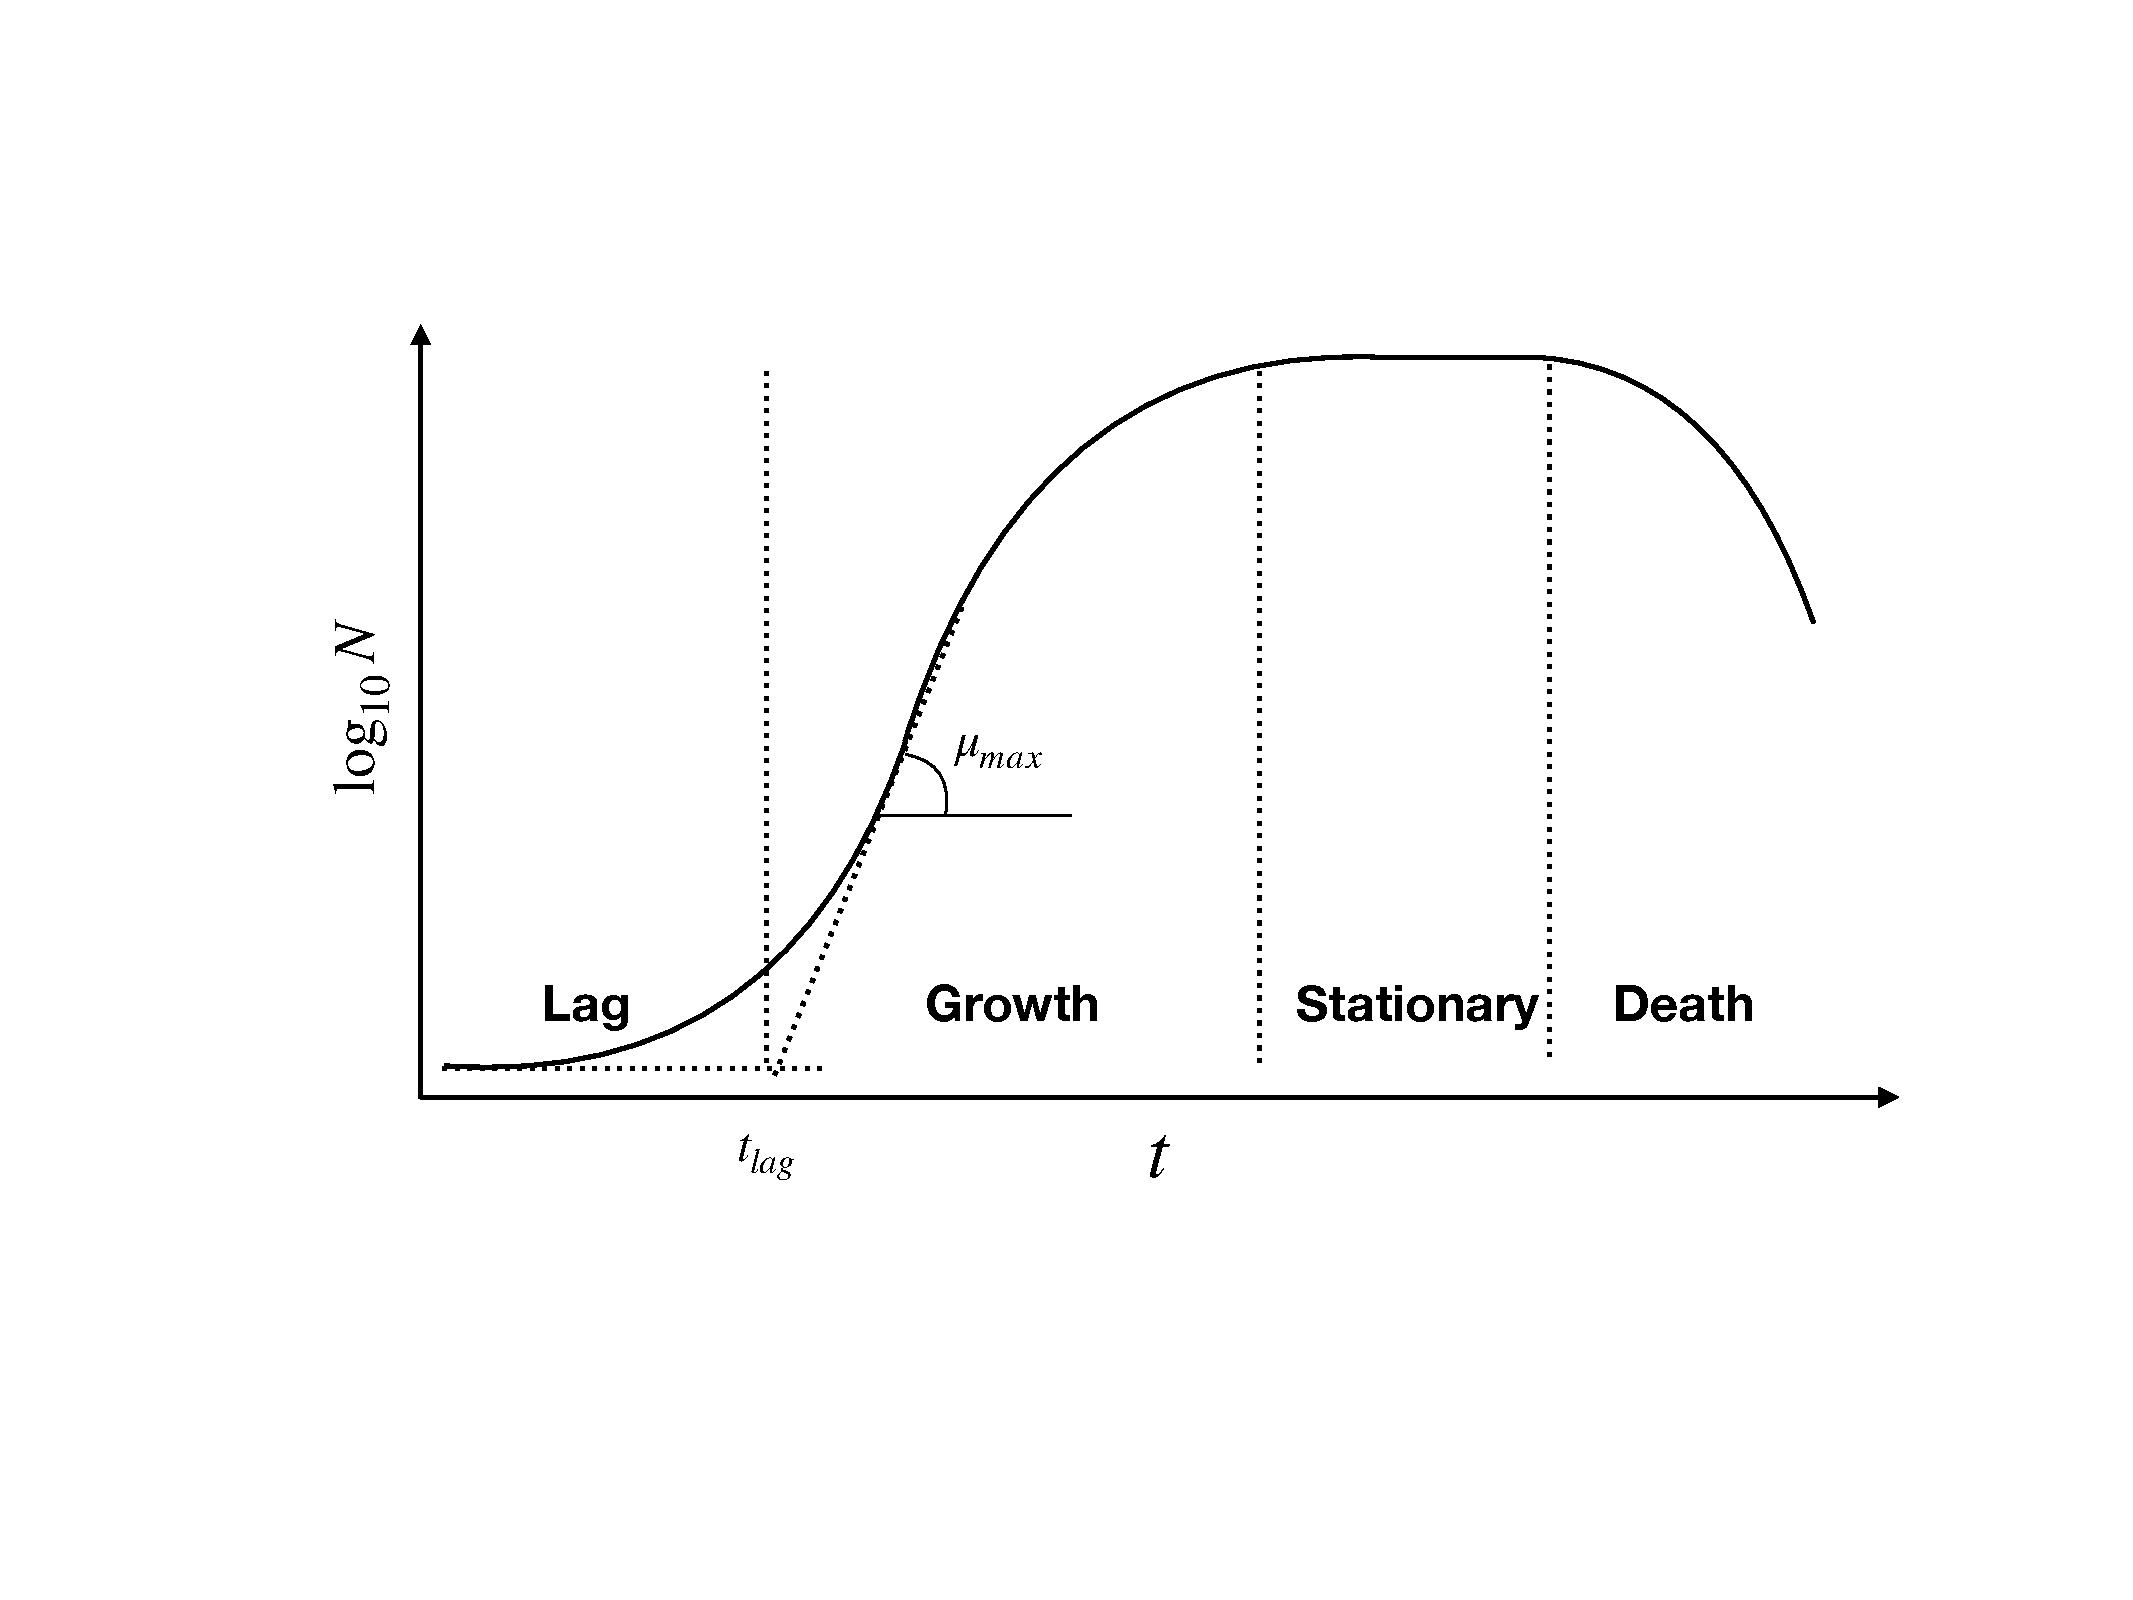
\includegraphics[scale=0.4]{growthcurve.pdf}
				\caption{Tipical growth curve showing the four phases: lag phase, exponential growth phase, stationary phase, and death phase. The geometrical interpretations of the growth rate and lag time are also shown.}
				\label{fig:growthcurve}
			\end{figure}
			Biological information can be extracted from the values of the parameters resulting from the model fits. Furthermore, the dependance of these parameters on external factors such as temperature $ T $, water activity $ a_w $, or pH can also be studied by using secondary models. Many studies have been conducted aiming to model the dependance of $ \mu_{max} \sim T $ \cite{Ratkowsky1982, Phillips1987, Stannard1985, DaSilva2018, Zwietering1991, Bernhardt2018, Lactin1995, Valik2013, Logan1976}.  A widely used group of secondary models that model this dependance are the thermal performance curves (TCP) (see figure \ref{fig:TCP_example}). In this work, the Lactin-2 model (see equation \ref{eq:Lactin-2}) is used to model the dependance of $ \mu_{max} $ on $ T $ for seven species on the genus \textit{Arthrobacter}.\\
			\begin{figure}[h]
				\centering
				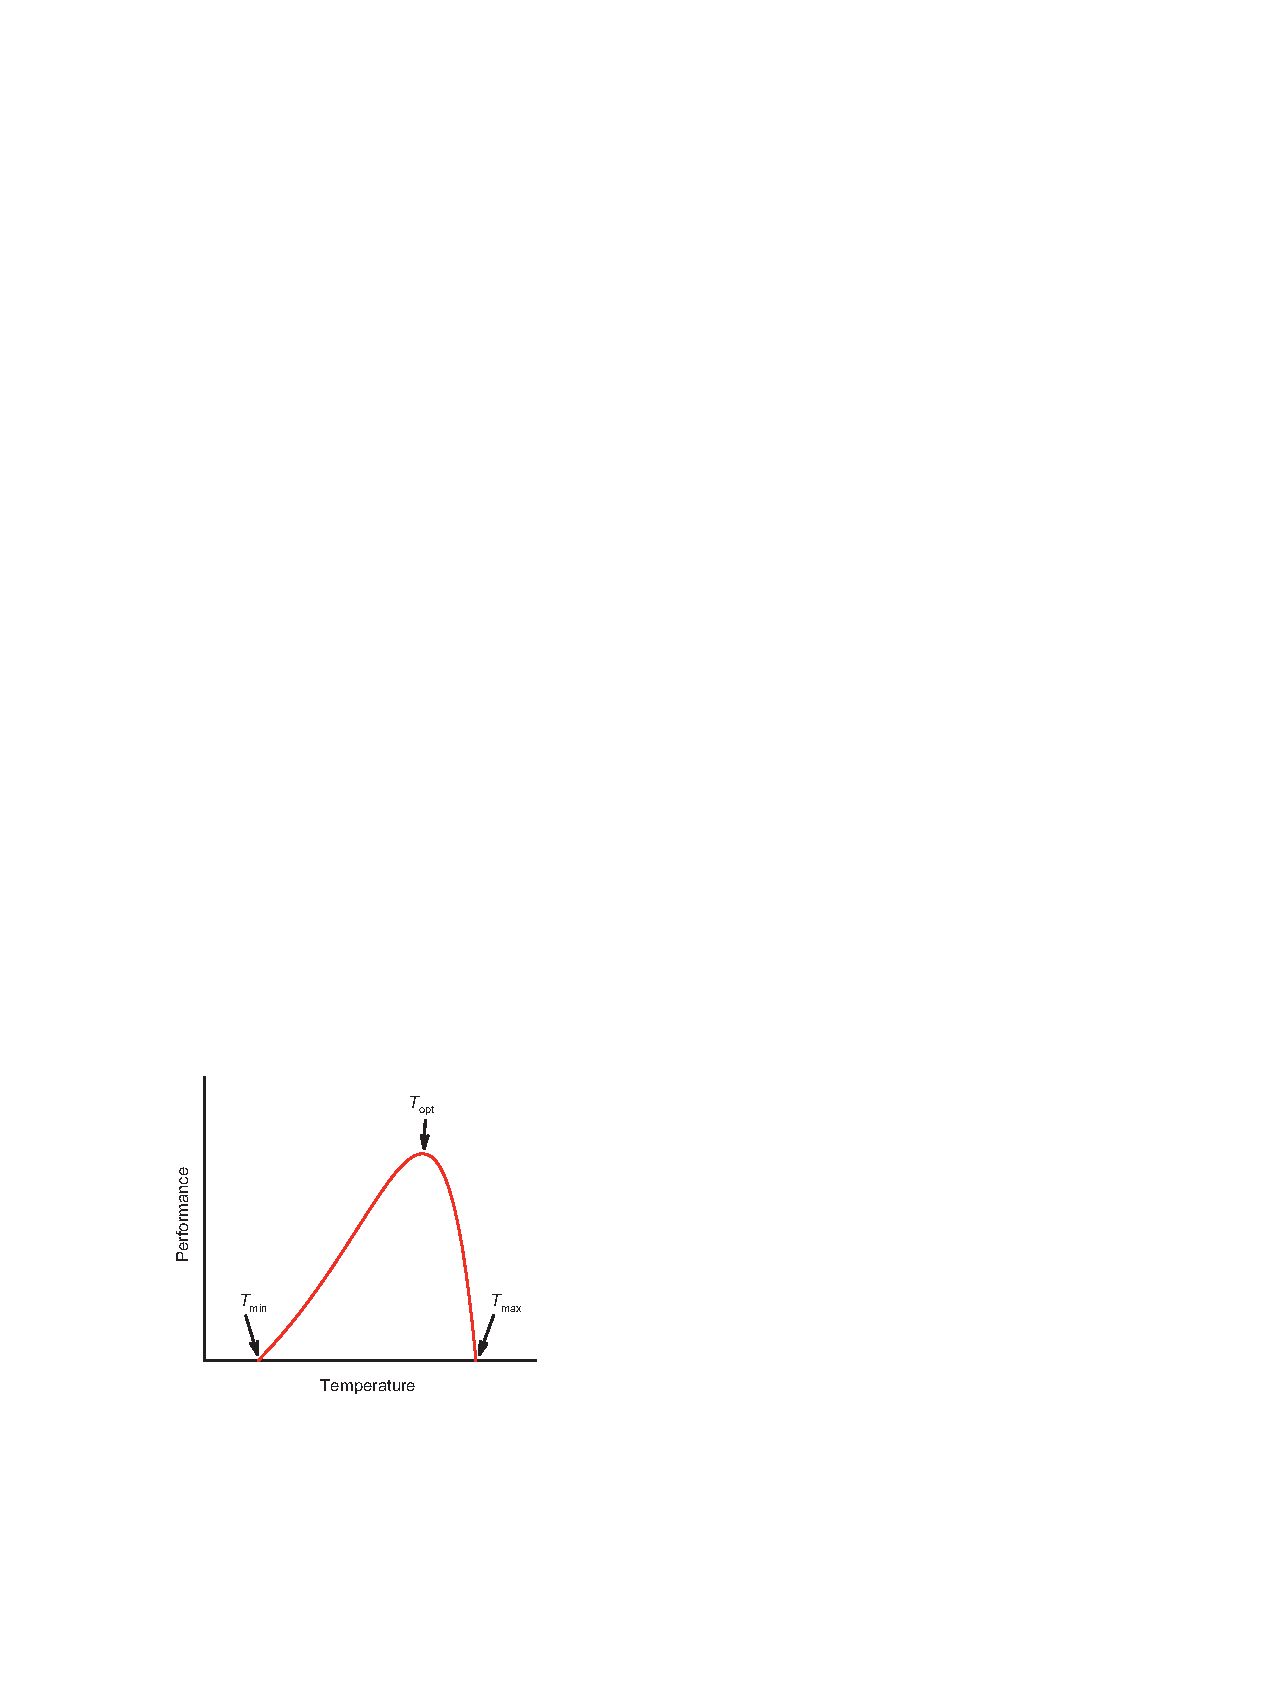
\includegraphics{TCP_example.pdf}
				\caption{General shape of a thermal performance curve. The thermal optimum $ T_{opt} $ defines the temperature at maximum performance. The critical thermal minimum ($ CT_{min} $) and maximum ($ CT_{max} $) are temperatures with thermal performance zero; they define the limit of an organism's thermal niche. The figure is taken from \cite{Krenek2011}.}
				\label{fig:TCP_example}
			\end{figure}
			We aim to address the continuity of psychrophilic and mesophilic growth characteristics in the genus Arthrobacter. Previous work on this topic \cite{ROTH1962} reported: "[...] no sharp cutoff point between growth-temperature requirements of psychrophilic and mesophilic bacteria". Here, we rigorously show such experimental observation by inspecting the distribution of fitted $ T_{opt} $ across species.\\
			
			\section{Methods}\label{methods}
			
			In this section, we explain the details of the data, present, and briefly discuss the tested models, summarize the workflow of the mini-project code as a whole, and motivate the use of each computing tool we employed.\\
			
			The data comes from a collection of 10 papers written between 1962 and 2018 \cite{Bae2014, Bernhardt2018, Galarz2016, Gill1991, Phillips1987, ROTH1962, DaSilva2018, Sivonen1990, Stannard1985, Zwietering1994} where the population of 45 species of bacteria is measured at different times (h), temperatures (ºC) and mediums.  The populations are expressed in different units depending on the paper, i.e,  optical density measured at 535 nm (OD$_{535} $), number of bacteria (N), colony-forming unit (CFU) and dry weight (DryWeight). Grouping datasets of population versus time for each temperature, species and medium yields 301 bacterial growth curves to which we can fit our models.\\
			After taking the $ \log_{10} $ of the population values, seven models are fit to the growth curves; exponential (which turns into linear after logging the population), quadratic , cubic, logistic \cite{Pearl1920, Verhulst1838}, Gompertz \cite{Zwietering1990}, Baranyi \cite{Baranyi1994} and Buchanan \cite{Buchanan1997} (figure \ref{all_models}). Refer to section \ref{subsec:modelequations} to see the mathematical form of each model. As seen in figure \ref{all_models}, we are fitting four linear models (linear, quadratic, cubic, Buchanan) and three non-linear models (logistic, Gompertz, Baranyi). \\
			\begin{figure}[h]
				\includegraphics[width= \linewidth]{all_models.pdf}
				\centering
				\caption{Overview of fit of each model to a growth curve where they perfrorm best (they have the lowest AIC value of out of all models for that curve)}
				\label{all_models}
			\end{figure}
			
			The general workflow of this project has two modules: Module 1 (fitting of all bacterial growth curves and model selection), and Module 2 (analysis of the biological question).  Each module has 3 subdivisions: data preparation, fitting and storing results, and plotting. These modules, along with the \LaTeX \ code that produces the present document are glued together in a script that coordinates all the tasks to run the mini-project smoothly
			\subsection{Module 1}\label{subsec:module1}
			This module concerns the fitting of all growth curves to all models and the model selection.\\
			The first step in this module is the data preparation (\verb|data_preparation_1.R|), in which we log the data, deal with bad quality data, and repeated measurements. First, we decide to log our data ($N(t) $ $\rightarrow$ $y(t)$) because the fitting performance and number of iterations until convergence are enhanced.  This is because taking $ \log_{10} $ decreases the scale of population values, particularly those measured in N units, which can be $ \sim $ 10$^{10} $. The mathematical form of the models also changes when logging the populations. Second, we eliminate the outliers in the population data (only one value of -682) that don't have any biological meaning. Next, we deal with negative values closer to 0 by finding the minimum of those values and adding it to all population values. This assures that all elements are positive without losing any data points, which are very valuable for the fits. Adding a constant to our population values will modify some of the fit parameter estimations, specifically all the coefficients from the second and third-order degree polynomials, but more importantly, y$_0 $ and y$ _{max} $ from the exponential, logistic, Gompertz, Baranyi and Buchanan models. However, that does not affect our model selection, or our biological question, because none of these analyses depend on the value of the affected parameters. Third, we address the repeated measurements, which are only present in the growth curves of the species  \textit{Tetraselmis tetrahele}. This data consists of repeated measures of the population at different times. However, the times at which the population is measured slightly differ among each repetition. To deal with this we create the function \verb|binning| (stored in \verb|data_preparation_functions.R|) that groups the slightly different times (within a threshold of 0.25) into averaged time groups, $  \overline{t_i}$. We use the binning for the time vector to bin our population accordingly into a vector of averaged populations, {$\overline{y_i}$}. This procedure yields a unique averaged dataset $ \left(\overline{t_i}, \overline{y_i}\right) $ that substitutes the repeated measurements of growth curves. This is the reason why we fit 285 growth curves instead of 305.\\
			
			The second step of module 1 is the model fitting and storing of results (\verb|fit_store_models_1.py|). This process consists of (a) loading the data, (b) looping through each growth curve, (c) calculating initial values for all the models, (d) fit each model to the i$ ^{th} $ curve, and (e) storing results (parameter estimates, fit evaluations, AIC values, Akaike weights, and performance information) in a dictionary for later use in the analysis. \\
			Steps a) and b) are trivial to perform. The initial values (step c) are set to 1 for the polynomial models. The convergence of the non-linear fits depends on the initial parameter values being reasonably close to the actual best-fit parameter values. Thus, the initial estimation for $ y_{0} $ and $ y_{max} $ are the maximum and the minimum of the population data being fitted. We determine $ \mu_{max} $ and $ t_{lag} $ by isolating the growth phase, and fitting a line to it. For a detailed explanation of how do we isolate the growth phase, and why fitting a line to it provides us with good initial parameter estimations, refer to section \ref{subsec:initial_values}. Step d) is implemented using the non-linear least squares (NLLS) fitting method. For a brief discussion on the theory behind this method, refer to section \ref{subsec:non-linear least squares fitting}. The AIC is calculated in step e. The expression for the AIC is
			\begin{linenomath*}
				\begin{equation}
				AIC = -2\log\left(\mathcal{L}(\boldsymbol{\beta}|x)\right) + 2p
				\label{AIC_general}
				\end{equation}
			\end{linenomath*}
			
			where $ \mathcal{L} $ is the likelihood of the model, and $ p $ the number of parameters. Under the assumptions that (1) we are using least squares to minimize our residuals, and (2) the errors are normally distributed, the following holds.
			\begin{linenomath*}
				\begin{equation}
				\log\left(\mathcal{L}(\boldsymbol{\beta}|x)\right) = -\frac{n}{2}log\left(\frac{S}{n}\right) 
				\end{equation}
			\end{linenomath*}
			
			where $ n $ is the number of data and $ S $ the residual sum of squares. Substituting the latter in equation \ref{AIC_general} one obtains the expression used to calculate our AIC values. \\
			\begin{linenomath*}
				\begin{equation}
				AIC = n + 2 + n \log\left(\frac{2\pi}{n}\right) + n\log S + 2 p
				\end{equation}
			\end{linenomath*}
			
			The Akaike weights $ w_i $, where $ i  = (1, 2, ..., R)$ is the number of models, are calculated for the Gompertz, Baranyi and Buchanan models in the following way. \cite{Anderson2002}\\
			First, we calculate the AIC differences $ \Delta_i = AIC_i = AIC_{min}$ for each model. This allows us to calculate the likelihood of the model given the data as
			\begin{linenomath*}
				\begin{equation}
				\mathcal{L}(g_i|x) \propto \exp\left(-\frac 1 2 \Delta_i\right)
				\end{equation}
			\end{linenomath*}
			Such likelihoods represent the relative strenght of evidence for each model.
			Finally, normalizing $ \mathcal{L}(g_i|x) $ gives us a set of positive Akaike weights for each model
			\begin{linenomath*}
				\begin{equation}
				w_i = \frac{\exp\left(-\frac 1 2 \Delta_i\right)}{\sum\limits_{r = 1}^{R}\exp\left(-\frac 1 2 \Delta_r\right)}
				\end{equation}
			\end{linenomath*}
			The performance information (step e) provides the clasification \textit{best, succesful, poor, bad, fail} in figure \ref{fig:success_report}.  Classifying a fit as \textit{best, success, bad, or fail} is trivial, and it is explained in figure \ref{fig:success_report}. To understand how can a fit be classified as \textit{poor}, refer to section \ref{subsec:poor}.\\
			
			The third step of the first module is the plotting phase (\verb|plotting_1.R|). Using the results previously obtained we plot every growth curve in a different figure and overlay the top four fits to it, according to the AIC. The intensity of the color of each fitting curve is also based on its AIC value (see figure \ref{fig:non_constrained}). All these plots are saved to the results directory. A fitting performance map (figure \ref{fig:success_report}) is also generated here.
			\subsection{Module 2}
			This module deals with the biological question stated in section \ref{sec:introduction}. \\
			In the data preparation step (\verb|data_preparation_2.R|), we select all the species of the genus \textit{Arthrobacter} along with the temperature and the growth rate. Note that most of the fits to \textit{Arthrobacter} species were flagged as \textit{poor}. We perform model averaging to obtain model-averaged estimates of maximum growth rate for each species and temperature, ie
			\begin{linenomath*}
				\begin{equation}
				\hat{\mu}_{max} = \sum\limits_{i = 1}^{R} w_i\mu_{max, i}
				\end{equation}
			\end{linenomath*}
			In the end, we have a data frame with seven species, and five data points ($ T $, $ \hat{\mu}_{max} $) each. \\
			Secondly, we perform NLLS fitting (\verb|fit_store_models_2.py|) to each dataset using the thermal performance curve proposed by Lactin et al. in 1995 \cite{Lactin1995}, which is a modification of the 1976 Logan-6 model \cite{Logan1976}. For a brief discussion on the Lactin-2 model refer to section \ref{subsec:Lactin-2}. In this case, the initial values for the fitting were taken from the literature \cite{Lactin1995}. $ T_{opt} $ is calculated for each species according to equation \ref{eq:Topt}.
			
			Third, we plot the results (\verb|plotting_2.R|) to generate figure \ref{fig:TCP}.
			\subsection{Computing tools}
			Modules 1 and 2 are written using Python and R. The latter one is used to perform the fitting using the LMFIT Python package \cite{Newville2014}. NumPy, Pandas \cite{Virtanen2020} and ProgressBar packages are also used for creating the models, saving the results, and implementing a progress bar, respectively. R is used to prepare data for analysis and plotting using ggplot2 \cite{Wickham2016}. RColorBrewer package is loaded to enable the \verb|YlOrRd| and \verb|RdYlBu| color palettes used in the fit plots and the fitting performance tilemap (figure \ref{fig:success_report}. The packages grid, and gridExtra are loaded to arrange multiple plots in one panel (figure \ref{all_models}).\\
			We choose to divide our work like this because Python is a faster language than R in general, so we use it to do the heavy lifting (fitting algorithms). However, R's flexibility and intuitive behavior when it comes to working with data frames are much better than Python's. Moreover, ggplot2 is the most powerful tool to generate publishable plots to our knowledge, which justifies using R for plotting instead of something else.\\
			The bash script \verb|run_MiniProject.sh| is used to glue all the scripts together in a working full version of the mini-project that runs in less than 90 seconds. We keep our work under version control with GitHub.
			
			\section{Results}
			Two categories of results are reported in this section: model selection and biological question results. \\
			Figure \ref{fig:success_report} summarizes the fitting performance and model selection results.
			\begin{figure}[h!]
				\includegraphics[width= \linewidth]{success_report.pdf}
				\centering
				\caption{Tile map summarizing the fitting performance and model selection results. Best fits are determined by selecting the model with the lowest AIC value for each growth curve. The amount of times (\%) that a model is the best candidate is specified in the x-axis. Success fits are convergent ones. Poor fits deal with data where the growth phase has $ \leq $1 data points. Bad fits were deemed as such when no recognizable growth pattern was found when performing a visual inspection. Fail fits converge to a local minimum instead of the global one, or don't converge at all.}
				\label{fig:success_report}
			\end{figure}
			The proportion of convergent fits decreases as the complexity of the model increases. Thus, all of the fits to the linear models converge. On the contrary, all the non-linear models fail once (logistic, Gompertz) or more times (Baranyi). Note that every time a non-linear fit fails, the best fit for that curve is not found among the other non-linear models, but instead in one of the linear models. The fits are generally better (in an AIC sense) in the non-linear models than in the linear ones. Particularly, the Gompertz model is the best most of the time (32\%), followed by the Baranyi model (24\%). The cubic model had a higher best model percent (19\%) compared to the Buchanan (16\%) and logistic (4\%) models. The linear (exponential) model was best the least amount of times (1\%) and the quadratic model was it 6\% of the times. Finally, a small proportion of the logistic, Gompertz, Buchanan and Baranyi fits are poor fits. Refer to section \ref{subsec:poor} to know how is this determined.\\
			\begin{figure}[h]
				\includegraphics[width= \linewidth]{TCP.pdf}
				\centering
				\caption{Fits of the Lactin-2 model to data from seven species of the genus \textit{Arthrobacter}. Fits for species \textit{Sp. 77} and \textit{Sp. 62} have been omitted for clarity.}
				\label{fig:TCP}
			\end{figure}
			The model-averaged $ \mu_{max} $  estimations are calculated, and plotted against $ T $. The Lactin-2 model is fitted for the data of each species (see figure \ref{fig:TCP}). Calculating $ T_{opt} $ for each species gives 19.2ºC for \textit{Sp 62}, 23.9ºC for \textit{Sp 77}, 27.4 ºC for \textit{Sp 88}, 28.3ºC for \textit{Arthrobacter Aurescens}, 34.8ºC for \textit{Arthrobacter Citreus}, 39.3ºC for \textit{Arthrobacter Simplex}, and 49.5ºC for \textit{Arthrobacter Globiformis}. 
			\section{Discussion}
			If there were no phenomena which were independent of all but a manageably small set of conditions, modeling in biology would be impossible \cite{Wigner1995}. Many models, each one considering a different set of relevant conditions, can successfully explain a given phenomenon.  To obtain the best estimates for the parameters of interest one can test competing models using model selection or null hypothesis testing. We believe that model selection is a better procedure to test competing hypotheses/models for several reasons. First, it allows for a comparison between more than two models (seven are analyzed in this work). Second, model selection is likelihood-based (as opposed to frequentist statistics based). Therefore, we can explicitly weigh the support for each model and even do model averaging if there is no obvious best model. This is something that cannot be done when using p-values to evaluate hypotheses because a p-value is not the probability that the null hypothesis is true, but instead, the degree of compatibility between a dataset and the null hypothesis \cite{RonaldL.Wasserstein, Kim2016}. This implies that the winning hypothesis is only implicitly accepted, by explicitly rejecting the null hypothesis. Moreover, the rejection of the null hypothesis is based on an arbitrary threshold of the p-value (0.05, 0.01). Overall, the model selection approach offers a more robust, objective, and meaningful way to test several competing models, than the conventional frequentist statistics method of calculating p-values. \\
			There are several approaches to model selection \cite{Johnson2004}, namely,  maximizing the quality of the fit, null hypothesis tests, and model selection criteria. The first one lacks a way of accounting for the complexity of the model, and the second one does not quantify the relative support among competing models, nor does it allow for comparison between more than 2 models. These limitations are overcome in model selection criteria. To determine the quality of the fits under these criteria, the most commonly used method is to calculate AIC or BIC. In this work, model selection was addressed using AIC. We chose to do so because the calculation of BIC assumes (a) the existence of a true model, (b) that the true model is within the examined pool of models, and (c) that each of the modes has the same probability of being the true one \cite{Johnson2004}. We deny assumption a), the existence of a true model, and consequently also assumptions b) and c) because we argue that  \textit{"all models are wrong, but some are useful"} \cite{Box1976, Box1979}. A true model, if attainable, would have to account for all the physical and biological processes that take place in the studied phenomena. This would make the model intractable due to its complexity. A good model should be simple enough to capture the behavior of the modeled process in an intuitive way, but not so simple to disregard essential mechanisms \cite{Chatfield1995}. \\
			When we calculate AIC values for each fit and model, we surprisingly find that the cubic model performs better than the logistic and Buchanan models. This is because the logistic and Buchanan only model the first three phases of a growth curve (figure \ref{fig:growthcurve}), and don't focus on a possible death phase. On the contrary, a third-degree polynomial can model decreasing populations after $ y_{max} $ has been reached. Fitting a growth model that accounts for a death phase \cite{Peleg2009, Baranyi1996} would eliminate this anomalous effect. However, those models are scarce in the food microbiology literature because most foods become inedible even before the mortality phase is reached \cite{Micha2011}, so there is no scientific incentive to come up with models that account for this.\\
			The logistic model has an unexpected very low \textit{best fit} percent. This result is caused by logging the logistic model. When we do so, the exponential growth that could reproduce the $ t_{lag} $ shape transforms into a straight line, which is unable to capture this pattern. From this point of view, it can be argued that fitting the logistic model in a linear scale is conceptually wrong since we are modeling a process of zero growth (lag phase), with slow exponential growth. Taking the logarithm of the data reveals this incongruence. To avoid it, some authors \cite{Micha2011, Zwietering1990} fit logged data with the linear logistic model. This is, in principle, a mistake, because when the data is rescaled the model must be rescaled too. However, the parameters of the logistic model can be recast to introduce a $ t_{lag} $ with no mechanistic interpretation \cite{Zwietering1990}. The validity of this resides in how important it is to be able to mechanistically interpret the parameters of a model. This question is an ongoing debate. Some authors even question if any mechanistic insights can be grasped from the value of parameters obtained by curve fitting alone \cite{Micha2011}. Being able to mechanistically interpret the parameters of a model depends on the purpose of your fitting. If it is merely for prediction, the simplest best model, (the Gompertz model in this work), should be the candidate of your choice. A  novel more robust method of obtaining parameter estimates for this purpose is model averaging. A discussion on why model averaging is used here is presented next, along with some remarks on the continuity of growth characteristics of some species in the genus \textit{Arthrobacter}.\\
			
			Most of the fits to \textit{Arthrobacter} species are poor. As described in section \ref{subsec:poor}, this implies that different models can perform well (have a hight $ \mathcal{L}(g_i|x) $) and still yield different values of the parameters. This inconvenience can be efficiently overcome by doing model averaging. Moreover, this approach is consistent with our skepticism about the existence of a true model, since our parameter estimates are a mixture of the parameter estimates of the tested models, weighted with the amount of support that we have for each of the candidates. \\
			The results from figure \ref{fig:TCP} point out the difficulty of establishing an arbitrary definition of a psychrophile. Among the seven members of the genus \textit{Arthrobacter} studied, no cut off region is apparent between psychrophiles and mesophiles. While we can clearly state that \textit{Sp 77, 88} and \textit{62} represent true mesophiles, according to the definition in \cite{INGRAHAM1958} and our $ T_{opt} $ results. There can also be no doubt that \textit{Simplex} and \textit{Globiformis} are true psychrophiles. However, there \textit{Citreus} and \textit{Aurescens} occupy the middle region of the \textit{Arthrobacter} temperature niche, and therefore, they cannot be categorized under any of the above categories. \\
			The species \textit{Simplex} and \textit{Globiformis} didn't have data in the region $ T > T_{opt} $. This caused the fit to yield parameters without biological meaning. To solve this problem, we impose for these two curves that $ T_{max} $ has to be no more than 60ºC. No mesophile was found in the literature \cite{Schiraldi2014} wich survives at higher temperatures than the imposed maximum. \\
			\section{Aknowledgements}
			We would like to thank Sam Turner for fruitful discussions regarding how to summarize the fitting performance and how to define poor fits. We also thank Hovig Artinian for his thoughtful thoughts on model averaging. 
			\newpage
			\section{Appendix}
			\subsection{Models}\label{subsec:modelequations}
			In this section, we provide all the explicit forms of the fitted models.\\
			The linear, quadratic, and cubic models have the form
			\begin{linenomath*}
				\begin{equation}
				y = y_0 + \mu_{max}t \quad , \quad     y = a + bt + ct^2 \quad, \quad y = \hat{a}+ \hat{b}t + \hat{c}t^2 + \hat{d}t^3
				\end{equation}
			\end{linenomath*}
			The logistic model reads
			\begin{linenomath*}
				\begin{equation}
				y =     \log_{10}\left(\dfrac{y_0y_{max}}{y_0 + (y_{max}-y_0)e^{-\mu_{max}t}}\right)
				\end{equation}
			\end{linenomath*}
			For the Gompertz model, we have
			\begin{linenomath*}
				\begin{equation}
				y = y_0 + (y_{max}-y_0)\exp\left(-\exp\left(e\mu_{max}\ \dfrac{(t_{lag}-t)}{\log_{10}(y_{max}-y_0)}+1\right)\right)
				\end{equation}
			\end{linenomath*}
			
			The Buchanan model can be expressed as 
			\[y = \left\{
			\begin{array}{lr}
			y_0 &  t < t_lag\\
			y_{max}  + \mu_{max}(t-t_{lag})&  t_{lag} \le t \le t_{max}\\
			y_{max} & t \geq t_{max}
			\end{array}
			\right.
			\]
			Finally, the Baranyi model has the form
			
			\begin{linenomath*}
				\begin{equation}                
				y_{max} + \log_{10}\left(\dfrac{-1 + e^{\mu_{max}t_{lag}} + e^{\mu_{max}t}}{e^{\mu_{max}t}-1+e^{\mu_{max}t_{lag}}10^{y_{max}-y_0}}\right)
				\end{equation}
			\end{linenomath*}
			
			
			\subsection{Initial values calculation}\label{subsec:initial_values}
			Given $ m $ data points $ D =  \left\{(x_1, y_1), (x_2, y_2), ... , (x_m, y_m)\right\} $ from a bacterial growth curve, and a tolerance $ \epsilon $ we perform the following steps to calculate initial estimations for the parameters $ \mu_{max} $, $ t_{lag} $. First, we calculate the $ m - 1 $ dimensional vector gradient between consecutive points as $ g_i = y_{i+1} - y_i $. Second, we find the maximum of that vector, $ g_{max} $. Third, we isloate the growing phase, $ D_{grow} = \left\{(\tilde{x}_1, \tilde{y}_1), (\tilde{x}_2, \tilde{y}_2), ... , (\tilde{x}_n, \tilde{y}_n)\right\} $ by selecting the datapoints in $ D $ whith $g_i \in [g_{max}(1-\epsilon), \ g_{max}(1+\epsilon)]$, with $ \epsilon = 0.3 $ by default.\\
			Fitting a line to $ D_{grow} $ yields the intercept and slope $ b $, $ m $ that can be used to calculate the initial parameters. The growth rate can be expressed as the slope of the growing phase scaled by a constant due to having logged the data, 
			\begin{linenomath*}
				\begin{equation}
				\mu_{max}  = p\log_{10}
				\end{equation}
			\end{linenomath*}
			
			The time lag has been traditionaly defined as the intersection of the tangents to the growth curve at the lag and exponential growth phases \cite{Micha2011}. This can be expressed mathematically, as 
			\begin{linenomath*}
				\begin{equation}
				t_{lag} = \frac{1}{m}(y_0 - b)
				\end{equation}
			\end{linenomath*}
			
			where $ y_0  $ is determined as described in section \ref{subsec:module1}
			\subsection{Non-linear least sqares fitting}\label{subsec:non-linear least squares fitting}
			Consider $ m $ data points $ \left\{(x_1, y_1), (x_2, y_2), ... , (x_m, y_m)\right\} $, and a model
			\begin{linenomath*}
				\begin{equation}
				y = f(x, \boldsymbol{\beta})
				\end{equation}
			\end{linenomath*}
			
			where $ \boldsymbol{\beta} = (\beta_1, \beta_2, ... , \beta_n) $ and $ m \geq n $. The aim is to find $ \boldsymbol{\beta}$ such as the model $ y $ fits best the given data points in the least square sense, i.e., the sum of squares
			\begin{linenomath*}
				\begin{equation}
				S = \sum_{i = 1}^{m} r^2_i
				\end{equation}
			\end{linenomath*}
			
			is minimized, where the residuals $ r_i $ are given by
			\begin{linenomath*}
				\begin{equation}
				r_i = y_i - f(x_i, \boldsymbol{\beta})
				\end{equation}
			\end{linenomath*}
			
			Finding the minimum value of $ S $ is equivalent to solve $ n $ equations where the partial derivative of $ S $ with respect the parameter $ \beta_j $, where $ j = 1, ..., n $ equals 0. Thus
			
			\begin{linenomath*}
				\begin{equation}
				\frac{\partial S}{\partial \beta_j} = 0    
				\end{equation}
			\end{linenomath*}
			This yields a non-linear systems of equations that, in general, does not have a closed solution. Consequently, initial values must be chosen for the parameters, so that they can be iteratively minimized. 
			\subsection{Classifying a fit as \textit{poor}}\label{subsec:poor}
			A fit to a bacterial growth curve with only 1 data point in the growing phase will yield poorly constrained values $ \mu_{max} $ and $t_{lag}$, because significantly different values of  these parameters for different models will all define a good fit. To ilustrate this, see figure \ref{fig:non_constrained}
			\begin{figure}[h!]
				\includegraphics[width= 0.8\linewidth]{non_constrained.pdf}
				\centering
				\caption{Example fit in which there is only 1 point in the growing phase, according to our method. The fit quality is very high ($ R^2 \ge 0.999 $). However, the values of $ \mu_{max} $ and $ t_{lag} $ for Gompertz, Buchanan and Baranyi models are, respectively, [0.045, 0.022, 0.061] (CFU h$^{-1}$) and [80.3, 45.1, 87.8] (h).}
				\label{fig:non_constrained}
			\end{figure}
			
			Given $ m $ data points $ D =  \left\{(x_1, y_1), (x_2, y_2), ... , (x_m, y_m)\right\} $ from a bacterial growth curve, a tolerance $ \epsilon $ and a bacterial growth model fit to that data, we flag it as \textit{poor} if there are 1 or none data points in the growth phase. To do this, we first isolate the growth phase and then count the elements in it.  Given the estimated parameters $ y_{0} $ and $ y_{max} $ from the fits, the growth phase $D_{grow} $ contains points of the form $ (x_i, y_i) / y_i \in [y_0 + \epsilon\ |y_0| , y_{max} - \epsilon \ |y_{max}]$. 
			
			\subsection{Lactin-2 model}\label{subsec:Lactin-2}
			The expression for the Lactin-2 model is 
			\begin{linenomath*}
				\begin{equation}\label{eq:Lactin-2}
				\mu(T) = \exp(\rho T) - \exp\left(\rho T_{max} - \frac{T_{max}-T}{\Delta T}\right) + \lambda    
				\end{equation}
			\end{linenomath*}
			
			The modifications respect to the Logan-6 model are; first, they omitted the paremeter $ \Psi $ which was originally defined as a physiological rate parameter at a given base temperature. Second, they incorporated the intercept parameter $ \lambda $, which forces the curve to intersect the abcissa at low temperatures and allows the estimation of $ T_{min} $.\\
			To find $ T_{opt} $ one finds the maximum of equation \ref{eq:Lactin-2}. Solving $ \frac{d\mu}{dT}  = 0$ yields the expression
			\begin{linenomath*}
				\begin{equation}\label{eq:Topt}
				T_{opt} = \frac{1}{\rho\Delta T  -1}\left[\rho T_{max} \Delta T - T_{max} + \Delta T \log\left(\frac{1}{\rho\Delta T }\right) \right]
				\end{equation}
			\end{linenomath*}
		\end{linenumbers}
		
		\newpage
		\bibliographystyle{unsrt}
		\bibliography{/Users/pablolechon/library}
	\end{document}
